\chapter{Multi-Robot Target Localization}



\section*{Problem Description}

Multi-robot target localization involves a team of robots collaboratively estimating the positions of one or more targets based on noisy 
sensor measurements. In this scenario a team of robots, each equipped with sensors for detecting targets within a limited sensing range, 
and these measurements are corrupted by noise. 
The goal is to design and implement a distributed strategy that enables the robots to cooperatively locate the targets and improve the 
accuracy of the estimation compared to individual measurements.


For visualization of the context, in general, we have the following.


\begin{figure}[h]
    \centering
    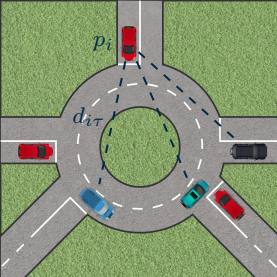
\includegraphics[width=0.4\textwidth]{img/Cap1/multi_robot_localization.png}
    \caption{Example of multi-robot target localization problem. A team of robots observing multiple targets. 
    Noisy measurements are 
    represented with dashed lines.}
    \label{fig:multi_robot_localization}
\end{figure}

\noindent
The problem is formulated as a distributed optimization task,
where we have a $N \in N $ robots that estimate the positions of multiple unknown targets in a cooperative mode, using only local, noisy distance measurements.
Each robot is assumed to be aware only of its own position and of the distances (corrupted by noise) to nearby targets, and can exchange information solely with its 
neighbors in a communication graph.


To tackle this challenge, the problem is approached in two stages:
\begin{itemize}
    \item \textbf{Task 1.1 - Distributed Consensus Optimization}: this focuses on the implementation and analysis of a distributed consensus optimization algorithm 
    Gradient Tracking which allows robots to collaboratively minimize a global objective function.
    \item \textbf{Task 1.2 - Cooperative Multi-Robot Target Localization}: this builds an algorithm to solve the specific localization problem, defining suitable 
    cost functions that encode the discrepancy between the measured distances and the estimated positions of the targets.
\end{itemize}

The proposed solution must be robust, scalable, and efficient, capable of handling different communication topologies and noisy sensor data, while 
guaranteeing convergence of the estimates across the network.

\subsection*{Code Structure Note}

For the sake of modularity and clarity, the implementation has been organized into multiple files, each responsible for a specific aspect of the project. 
The code is organized as follows:

\begin{itemize}
    \item \texttt{main.py}: Entry point of the simulations, used to set parameters and run both tasks.
    \item \texttt{utils\_graph.py}: File that contains utility functions for generating and handling different graph topologies (e.g., cycle, path, star,erdos\_renyi) 
    and computing Metropolis-Hastings weights.
    \item \texttt{utils\_visualization.py}: File dedicated to plotting the evolution of the cost function and gradients, and optionally animating robot movements.
    \item \texttt{utils\_world\_generation.py}: File for creating the simulated environment, including the generation of agents and targets within a bounded space.
    \item \texttt{gradient\_tracking.py}: File to implementation of the Gradient Tracking algorithm used in both tasks, with same different.
    \item \texttt{cost\_functions.py}: Definition of the local and global cost functions used in the optimization problem.
\end{itemize}

This modular structure enables the reuse of core components and makes the transition from consensus optimization (Task 1.1) to cooperative target localization (Task 1.2) 
seamless.



\section{Distributed Consensus Optimization}

\subsection{Problem Statement}
In this task, we address a distributed consensus optimization problem arising in multi-agent systems. The objective is to solve an unconstrained optimization problem of the 
form:

\begin{equation}
    \min_{z \in \mathbb{R}^d} \sum_{i=1}^N \ell_i(z),
\end{equation}
where:
\begin{itemize}
    \item \( z \in \mathbb{R}^d \) is the global decision variable to be optimized,
    \item \( N \in \mathbb{N} \) is the number of agents (robots),
    \item \( \ell_i: \mathbb{R}^d \rightarrow \mathbb{R} \) is a local objective function known only to agent \( i \).
\end{itemize}

Each agent \( i \) has access only to its own cost function \( \ell_i(z) \) and can communicate with a limited set of neighboring agents defined by a communication 
graph \( \mathcal{G} = (\mathcal{I}, {E}) \), where \( \mathcal{I} = \{1, \dots, N\} \) is the set of nodes and \( E \subseteq \mathcal{I} \times \mathcal{I} \) is the set 
of edges. 

\noindent
The goal is to design a distributed algorithm that allows all agents to cooperatively find a minimizer of the global cost function by exchanging information only 
with their immediate neighbors in the graph \( \mathcal{G} \).
\noindent
To evaluate the performance of the distributed consensus optimization algorithm, are implemented a different simulation. In particular, consider different types of
graph structures such as cycle, path, star, erdos\_renyi graphs to model the communication network among the agents. 

\noindent For each topology, the communication weights are defined using the \textit{Metropolis Hastings rule}, ensuring the resulting weight matrix is symmetric and 
doubly stochastic, which is essential for convergence guarantees.
\noindent
In this context, consensus optimization techniques are crucial as they enable a collective decision-making process, ensuring that all agents converge to a 
common optimal solution through local computations and communications.


\subsection{Algorithm Implementation}


\begin{tcolorbox}[colback=white,colframe=black!75!black,title=ADD IMPLEMENTATION ]

\end{tcolorbox}


\section{Cooperative Multi-Robot Target Localization}

In the second part of the task, leveraging the work done in Task 1.1, the goal is to implement the \textit{Gradient Tracking} algorithm to enable a fleet of 
robots to cooperatively localize multiple targets in the environment.

\noindent
The main objective is to estimate the positions of multiple targets by using noisy distance measurements from the robots to the targets, while ensuring consensus 
among the robots on the final estimates.

\subsection{Problem Statement}
The scenario involves a set of \( N \) robots, each with an unknown position \( p_i \in \mathbb{R}^d \), and \( N_T \) static targets whose positions are to be estimated.
\noindent
Each robot obtains noisy measurements of its distances \( d_{i\tau} \in \mathbb{R}_{\geq 0} \) to each target \( \tau = 1, \ldots, N_T \). The robots aim to collectively 
minimize a local cost function defined as: 
\begin{equation}
    f_i(z) = \sum_{\tau=1}^{N_T} \left( d_{i\tau}^2 - \| z_\tau - p_i \|^2 \right)^2,
\end{equation}
    
where \( z = \mathrm{col}(z_1, \ldots, z_{N_T}) \in \mathbb{R}^{d N_T} \) is the concatenated vector of target position estimates \( z_\tau \in \mathbb{R}^d \).

By implementing the Gradient Tracking algorithm, the robots iteratively update their local estimates while exchanging information with their neighbors, achieving 
consensus on the target locations. 

\noindent
So the algorithm minimize the local cost functions cooperatively, allowing the robots to share information and iteratively update their estimates.



\subsection{Algorithm Implementation}


\begin{tcolorbox}[colback=white,colframe=black!75!black,title=ADD IMPLEMENTATION ]

\end{tcolorbox}